\documentclass[12pt]{scrartcl}                                                      % 'Artikel' Dokumentenklasse und Standardschriftgröße  
\usepackage[paper=a4paper,left=2.5cm,right=2.5cm,top=2.5cm,bottom=2.5cm]{geometry}  % Setzt das Papierformat und den Rand auf 2.5cm


\setlength{\parindent}{0.5 em}                                                         % Setzt die Einrückung von Absätzen auf gegebenen Abstand
\usepackage[onehalfspacing]{setspace}                                               % Legt Zeilenabstand fest


\usepackage[T1]{fontenc}                                                            % Legt FontKodierung fest
\usepackage[utf8]{inputenc}                                                         % Legt Zeichenkodierung fest

\usepackage[ngerman]{babel}                                                         % Deutsche Rechtschreibung
%\usepackage[ngerman]{varioref}                                                      % Versieht Referenzen mit Bezeichnung des Objektes
\usepackage{lmodern}                                                                % Empfohlener T1-Font für deutsche Texte
\usepackage[backend=biber, style=numeric-verb]{biblatex}
\usepackage[babel,german=quotes]{csquotes}
%%%%%%%%%%%%%%%%%%%%%%%%%%%%%%%%%%%%%%%%%%%%%%%%%%%%%%%%%%%%%%%%%%%%%%%%%%

\usepackage{fancyhdr}                                                               % Ermöglicht detailierte Bearbeitung der Kopf- und Fußzeile
\fancyhf{} 	                                                                        % Setzt Kopf und Fußzeile zurück 
\setlength{\headheight}{28.0pt}                                                     % Höhe der Kopfzeile
\setlength{\footskip}{18.0pt}                                                       % Höhe der Fußzeile

\renewcommand{\headrulewidth}{.5 pt}                                                 % Dicke des Kopfzeilentrennstrichs
\renewcommand{\footrulewidth}{.5 pt}                                                 % Dicke des Fußzeilentrennstrichs

\lhead{\textbf{\VNr\\ \VN}}                                                                   % Angabe Links-Oben
%\chead{}                                                                           % Angabe Mitte-Oben
\rhead{\VD}                                                                      % Angabe Rechts-Oben
\lfoot{\Namen}                                                                           % Angabe Links-Unten
\cfoot{\textbf{\thepage\ von \pageref{LastPage}}}                                   % Angabe Mitte-Unten
\rfoot{\Emails}                                            % Angabe Rechts-Unten

%%%%%%%%%%%%%%%%%%%%%%%%%%%%%%%%%%%%%%%%%%%%%%%%%%%%%%%%%%%%%%%%%%%%%%%%%%
\usepackage{scrdate}
\usepackage{lastpage}                                                               % Macht die letzte Seitenzahl referenzierbar mit \pageref{Lastpage}
\usepackage{hyperref}
\hypersetup{hidelinks}                                                              % Ermöglicht Verlinkungen im Dokument

%%%%%%%%%%%%%%%%%%%%%%%%%%%%%%%%%%%%%%%%%%%%%%%%%%%%%%%%%%%%%%%%%%%%%%%%%%

\usepackage[sumlimits,intlimits,namelimits]{amsmath}                                % Fügt mathematische Symbole hinzu, setzt Grenzen, Limiten und Indizes unter das Symbol und nicht dahinter
\usepackage{amssymb}                                                                % Fügt Symbole wie z.B. Zahlenmengen wie $\mathbb{R}$ hinzu 
\usepackage{amsthm}                                                                 
\usepackage{amsfonts}                                                               % Fügt Font für Mathematikumgebung hinzu

\usepackage{empheq}                                                                 % Stellt verbesserte Gleichungsumgebung bereit \begin{empheq}[<Aussehen>]{<Umgebungstyp>} ... \end{empheq}
%test
\usepackage[version=3]{mhchem}                                                     % Stellt chemische Struktur und Summenformeln bereit \ce{<Summenformel>}
%\usepackage{chemfig}                                                               % Stellt chemische Valenzstrichformeln fürganze Moleküle bereit \chemfig{<Molekül-Aufbau>}

\usepackage{siunitx}                                                                % Stellt eine verbesserte Formatierung von größen mit Einheiten zur Verfügung  
\sisetup{locale = DE%
%,prefixes-as-symbols = false %
}                                   % Setzt das 'Mal'-Zeichen auf \cdot und das Dezimaltrennzeichen auf ',' 
                                                                                    % und ersetzt Prefixe wie '\kilo' mit der entsprechenden Zehnerpotenz
\sisetup{separate-uncertainty = true}                                               % Ermöglicht vereinfachtes eintragen von Unsicherheiten '42.6(4)' --> '42.6 +/- 0.4'                                                                                 

\usepackage{textcomp}                                                               % Fügt extra Symbole hinzu   
\usepackage[b]{esvect}                                                              % Fügt verbesserte Vektorpfeile hinzu \vv{<Vektorname>} 
\usepackage{xfrac}
\usepackage{array}
\usepackage{commath}																% Fügt Differentialoperatoren und -quotienten ein 
%%%%%%%%%%%%%%%%%%%%%%%%%%%%%%%%%%%%%%%%%%%%%%%%%%%%%%%%%%%%%%%%%%%%%%%%%%

\usepackage{graphicx}                                                               % Ermöglicht das Einbinden Grafiken '\includegraphics[<Optionen>]{<Grafikpfad>}' und Veränderungen im Text, wie z.B. Schriftfarbe 
\usepackage{floatflt}                                                         % Fügt Möglichkeit für text umflossende Grafiken und Tabellen hinzu \begin{floating<figure/table>}[option]{width} ... \caption ... \end{floatingfigure}
%\usepackage{subfig}                                                                % Ermöglicht das Hinzufügen von Unterabbildung zu einer Abbildung
\usepackage{wrapfig}
\usepackage{tikz}                                                                   % Ermöglicht Zeichnungen im Dokument \begin{tikzpicture} ... \end{tikzpicture}
\usetikzlibrary{arrows}                                                             % Fügt zusätzlichen Pfeilspitzen hinzu
%\usepackage{booktabs}
%%%%%%%%%%%%%%%%%%%%%%%%%%%%%%%%%%%%%%%%%%%%%%%%%%%%%%%%%%%%%%%%%%%%%%%%%%

\usepackage[normalem]{ulem}                                                         % Fügt verbesserte Unterschtreichungen hinzu, z.B. doppelt, gezackt, gewellt, etc.
\usepackage{enumitem}                                                               % Ermöglicht detailierte Einstellungen an Aufzählungssymbolen
%\usepackage{slashbox}                                                              % Ermöglicht das Einfügen mehrerer Einträge in eine Tabellenzelle, getrennt von einem '\' \backslashbox{<Eintrag unten-links>}{<Eintrag oben-rechts>} TIPP: Leerzeichen

\usepackage[font=small,labelfont=bf]{caption}
\usepackage{pifont}																    % Fußnoten mit Zahlen in Kreisen
\renewcommand\thefootnote{\ding{\numexpr171+\value{footnote}}}
%%%%%%%%%%%%%%%%%%%%%%%%%%%%%%%%%%%%%%%%%%%%%%%%%%%%%%%%%%%%%%%%%%%%%%%%%%

\title{} 
\author{} 
\addbibresource{../globales/latex/Literatur.bib}
%%%%%%%%%%%%%%%%%%%%%%%%%%%%%%%%%%%%%%%%%%%%%%%%%%%%%%%%%%%%%%%%%%%%%%%%%%

\pagestyle{fancy}                                                                   % Anwenden des Erweiterten Seitenlayouts

%\renewcommand{\thefootnote}{}
%\setlength{\footnotesep}{2cm}
\setlength{\skip\footins}{2cm}                                                      % Abstand zwischen Text und Fußnoten
%\setlength{\itemsep}{7.5pt}

\newcolumntype{C}{ >{\centering\arraybackslash} m{2.5 cm}}



\renewcommand{\i}{\ensuremath{\textsl{i}}}
\newcommand{\e}{\ensuremath{\textsl{e}}}
\renewcommand{\Im}{\mathrm{Im}\,}
\renewcommand{\Re}{\mathrm{Re}\,}


%\DeclarePairedDelimiter{\abs}{\lvert}{\rvert}
\DeclarePairedDelimiter{\mean}{\langle}{\rangle}

%%%%%%%%%%%%%%%%%%%%%%%%%%%%%%%%%%%%%%%%%%%%%%%%%%%%%%%%%%%%%%%%%%%%%%%%%%
\usepackage[ngerman]{cleveref}
\crefformat{equation}{(#2#1#3)}
\crefrangeformat{equation}{(#3#1#4) bis~(#5#2#6)}

\usepackage{xcolor}


\newcommand{\VNr}{V206}                                                             % Makro für die aktuelle Versuchsnummer
\newcommand{\VN}{Die Wärmepumpe}                                                    % Makro für den aktuellen Versuchsnamen
\newcommand{\VD}{07. November 2013}                                                 % Makro für das Versuchsdatum
%\renewcommand{\thefootnote}{\Roman{footnote}}
%\renewcommand{\theequation}{\Roman{equation}}
\begin{document}
	\section{Einleitung}\label{sec:Einleitung}
		\Huge \textcolor{red}{EINLEITUNG}
\normalsize
	

%	\section{Vorbereitungsaufgaben}
	
	
	
	\section{Theorie}\label{sec:Theorie}
		Der Lock-In-Verstärker kann stark verrauschte Signale messen, dazu wird das verrauschte Signal in mehreren Schritten bearbeitet. Als erstes wird das verrauschte Signal im Preamplifier verstärkt. Anschließend wird das Signal von Frequenzen, die stark von einer beim Bandpassfilter einstellbaren Frequenz abweichen, befreit.
Im nächsten Schritt wird das Signal in einem Mischer mit einem
Referenzsignal, welches eine einstellbare Phase besitzt, multipliziert. Die Frequenz des Referenzsignals wird dabei der des zu messenden Signals angeglichen. Das Referenzsignal ist hier eine Sinusspannung. 
Damit das Referenzsignal hat die Form:

\begin{equation}
  \label{eq:ref}
  U_{ref} = \frac{4}{\pi} \left( \sin(\omega t) + \frac{1}{3} \sin(\omega t) + \frac{1}{5} \sin(\omega t) + ... \right)
\end{equation}

Die Formel für das zu messende Signal ist gegeben durch:

\begin{equation}
  \label{eq:sig}
  U_{sig} = U_{0} \sin(\omega t)
\end{equation}

Die Multiplikation der beiden Signale $U_{sig}$ und $U_{ref}$ ergibt:

\begin{equation*}
  U_{sig} \times U_{ref} = \frac{2}{\pi} U_{0} \left(1 - \frac{2}{3} \cos(2\omega t) + \frac{2}{15} \cos(4\omega t) + \frac{2}{35} \cos(6\omega t) + ... \right)
\end{equation*}

Da der Tiefpass nur niedrige Frequenzen durch lässt, ergibt sich die Form von $U_{out}$, nach Mischer und Tiefpass.

Zusätzlich muss noch der Phasenunterschied $\phi$ beachtet werden, sollte einer vorliegen, muss dieser mit betrachtet werden.

\begin{equation}
  \label{eq:Uout}
   U_{out} = \frac{2}{\pi} U_{0} \cos(\phi)
\end{equation}

Das endgültige Signal ist damit eine Gleichspannung, die proportional zum
Produkt der Amplituden der Referenzspannung und des Signals $\cos(\phi)$ ist.

	
	
	\section{Durchführung}\label{sec:Durchführung}
		\input{Latex/Durchführung.tex}
	
	
	\section{Auswertung}\label{sec:Auswertung}
		Im Folgenden sind die während des Versuchs aufgenommenen Messwerte und die aus diesen 
berechneten Größen tabellarisch dargestellt. An entsprechender Stelle sind Erklärungen
zu den zu den Werten und Rechnungen gegeben.\\

\subsection{Bestimmung der Verdampfungswärme\\ bei Drücken unter einem bar}
\label{sec:gemittelteVerdampfungswärme}
	In \autoref{tab:DataI} sind die, für diese Auswertung verwendeten, Messwerte für Temperatur und 
	Druck dieses Teilversuches zu finden. Dabei sind die angegebenen Messunsicherheiten der Temperaturen
	durch die Einteilung Skala des Thermometers und die Unsicherheiten der Drücke durch die Anzeigegenauigkeit 
	des verwendeten Barometers bestimmt. Letztere änderte sich im Verlauf des Versuchs, beziehungsweise
	musste im Verlauf des Versuchs angepasste werden, da sich die Fluktuation der auf dem Barometer angezeigten
	Messwerte vergrößerte.  
	
		\begin{table}[!h]
			\centering
			\begin{tabular}{|c|c||c|c|}
				\hline
				    Temperatur      &       Druck       &      Temperatur      &       Druck       \\
				$T\,[\si{\kelvin}]$ & $p\,[\si{mbar}] $ & $ T\,[\si{\kelvin}]$ & $ p\,[\si{mbar}]$ \\ \hline\hline
				   %\num{333(1)}     &   \num{244(1)}    & 
				   %\num{335(1)}     &   \num{260(1)}    &    
				   %\num{337(1)}     &   \num{275(1)}    &     
				   %\num{339(1)}     &   \num{291(1)}    &     
				   %\num{341(1)}     &   \num{310(1)}    
				   %\num{343(1)}     &   \num{332(1)}    
				   %\num{345(1)}     &   \num{349(1)}    
				   %\num{347(1)}     &   \num{374(1)}    
				   \num{349(1)}     &   \num{400(1)}    &    \num{361(1)}     &   \num{643(10)}   \\ 
				   \num{351(1)}     &   \num{429(1)}    &    \num{363(1)}     &   \num{694(10)}   \\
				   \num{353(1)}     &   \num{467(1)}    &    \num{365(1)}     &   \num{747(10)}   \\
				   \num{355(1)}     &   \num{506(10)}   &    \num{367(1)}     &   \num{796(10)}   \\
				   \num{357(1)}     &   \num{553(10)}   &    \num{368(1)}     &   \num{821(10)}   \\
				   \num{359(1)}     &   \num{591(10)}   &    \num{369(1)}     &   \num{851(10)}   \\ \hline
			\end{tabular}
			\caption{Werte der Messung bei $p < \SI{1}{bar}$ \label{tab:DataI}}
		\end{table}
	
	Diese Messwerte sind zusammen mit einer Regressionskurve der Form \eqref{eq:pT_exp} in \autoref{fig:pT1}
	aufgetragen, die wegen der halblogarithmischen Skalierung und der Definition $x := \tfrac{1}{T}$ eine Gerade 
	der Form \eqref{eq:pT_ln} darstellt.

	\begin{figure}[!h]
		\centering
		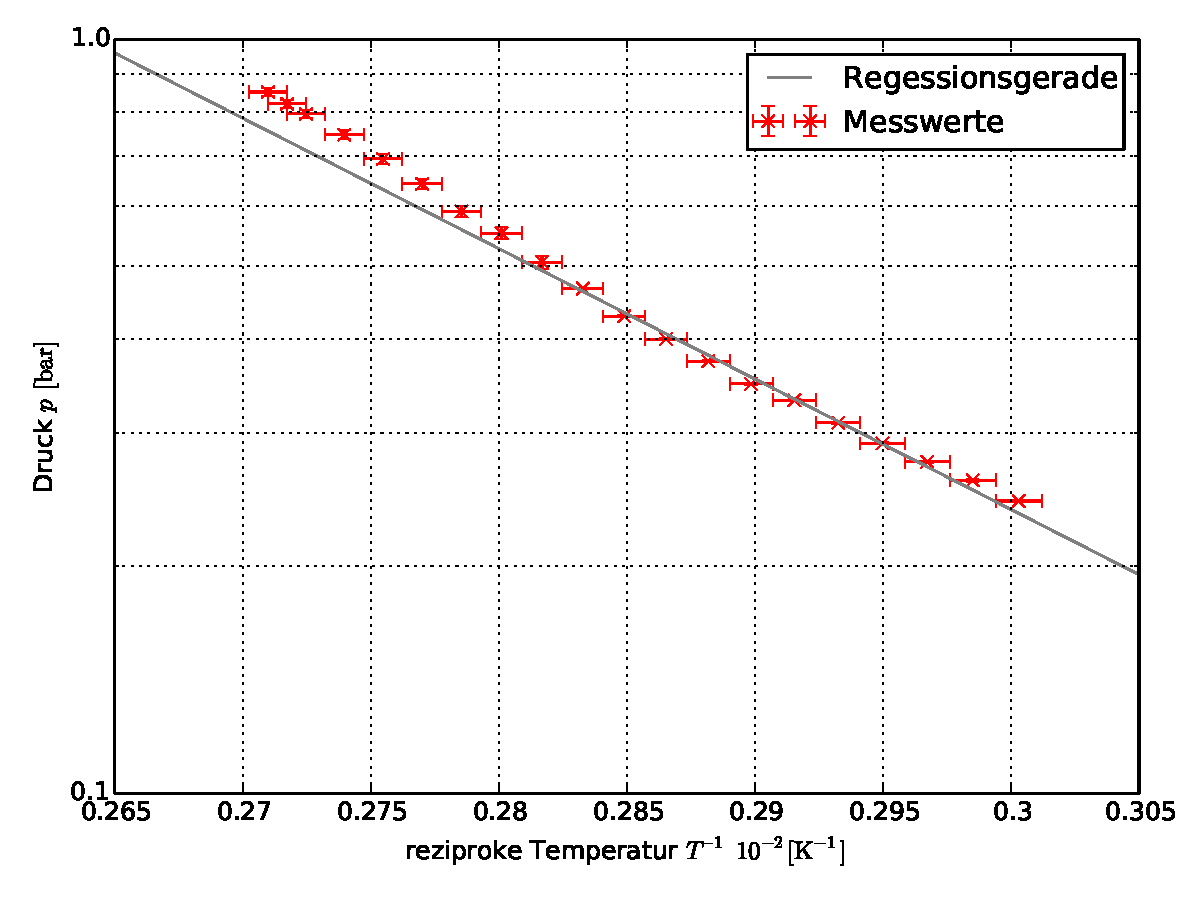
\includegraphics[scale=0.75]{Grafiken/Messreihe_1.pdf}
		\caption{Halblogarithmische Darstellung der Messwerte mit Regressionsfunktion}
		\label{fig:pT1}
	\end{figure}   
	
	Die mit Hilfe der Python Bibliothek \emph{SciPy} \cite{SciPy} bestimmten Parameter der Regerssionsfunktion 
	\begin{empheq}{equation}
		f(x) = Ax + B
	\end{empheq}
	sind:
	\addtocounter{equation}{-1}
	\begin{subequations}
		\begin{empheq}{align}
			\label{eq:A}
			A &= \SI{-0.0491(5)}{\bar\kelvin}\\
			\label{eq:B}
			B &= \SI{13(11)}{\bar}
		\end{empheq}
	\end{subequations} 
	
	 Mit der Steigung  $A = - \tfrac{L}{R}$ und der allgemeinen Gaskonstante $R = \SI{8.314}{\joule\per\mol\per\kelvin}$  \cite{SciPy} lässt
	 sich die Verdampfungswärme aus \eqref{eq:A} zu
	 
	\begin{empheq}{equation*}
	 		\label{eq:L}
	 		L = \SI{4.09(4)e04}{\joule\per\mole}
	\end{empheq}
	berechnen. Der angegebene Fehler wurde dabei über \eqref{eq:std_L} bestimmt. 
	
\subsection{Bestimmung der inneren Verdampfungswärme}
\label{sec:innereVerdampfungswärme}
Für die äußere Verdampfungswärme $L_{a}$ erhält man unter Verwendung der allgemeinen
Gasgleichung \eqref{eq:allgGas} und der Annahme $V_{F} << V_{D} $ die Näherung
\begin{empheq}{equation}
 	\label{eq:L_a}
 	L_{a} = RT.
\end{empheq}
Bei der gegebenen Temperatur $T = \SI{373}{\kelvin}$ ergibt sich damit die notwendige 
Energie, um das Volumen $V_{F}$ auf $V_{D}$ zu vergrößern zu
\begin{empheq}{equation*}
	 	L_{a} =  \SI{3101}{\joule\per\mole}\;.
\end{empheq}  
Aus der gesamten $L$ und  äußeren Verdampfungswärme $L_{a}$ lässt sich mit \eqref{eq:L_i}
die innere Verdampfungswärme bestimmen.

Durch Skalierung mit der Avogadro-Konstante 
$N_{A} = \SI{6.022e23}{\per\mole}$ \cite{SciPy} und Umrechnung in $\si{\eV}$\footnote{$\SI{1}{\eV} = \SI{1.602e-19}{\joule}$ \cite{SciPy}},
erhält man die für die Verdampfung eins einzelnen Wassermoleküls benötigte Energie
\begin{empheq}{equation*}
		 	L_{i} =  \SI{0.391(4)}{\eV}\;
\end{empheq} 
deren Fehler mit Hilfe von \eqref{eq:std_Li} berechnet wurde.
	
\subsection{Bestimmung der Temperaturabhängigkeit\\ der Verdampfungswärme}
\label{sec:Auswertung_TempAbhängigkeit}
	Die für die folgende Auswertung verwendeten Werte für Druck und Temperatur der zweiten Messung, sind in
	\autoref{tab:DataII} dargestellt. 
	
	\begin{table}[!h]
		\centering
		\begin{tabular}{|c|c||c|c|}
			\hline
			    Temperatur      &      Druck       &     Temperatur      &      Druck       \\
			$T\,[\si{\kelvin}]$ & $p\,[\si{\bar}]$ & $T\,[\si{\kelvin}]$ & $p\,[\si{\bar}]$ \\ \hline\hline
			  \num{343.2(1)}    &  \num{0.90(1)}   &   \num{413.2(1)}    &  \num{2.33(1)}   \\
			  \num{348.2(1)}    &  \num{0.92(1)}   &   \num{418.2(1)}    &  \num{2.72(1)}   \\
			  \num{353.2(1)}    &  \num{0.93(1)}   &   \num{423.2(1)}    &  \num{3.18(1)}   \\
			  \num{358.2(1)}    &  \num{0.95(1)}   &   \num{428.2(1)}    &  \num{3.72(1)}   \\
			  \num{363.2(1)}    &  \num{0.97(1)}   &   \num{433.2(1)}    &  \num{4.36(1)}   \\
			  \num{368.2(1)}    &  \num{1.01(1)}   &   \num{438.2(1)}    &  \num{5.12(1)}   \\
			  \num{373.2(1)}    &  \num{1.05(1)}   &   \num{443.2(1)}    &  \num{5.93(1)}   \\
			  \num{378.2(1)}    &  \num{1.10(1)}   &   \num{448.2(1)}    &  \num{6.84(1)}   \\
			  \num{383.2(1)}    &  \num{1.17(1)}   &   \num{453.2(1)}    &  \num{7.93(1)}   \\
			  \num{388.2(1)}    &  \num{1.26(1)}   &   \num{458.2(1)}    &  \num{9.17(1)}   \\
			  \num{393.2(1)}    &  \num{1.37(1)}   &   \num{463.2(1)}    &  \num{10.54(1)}  \\
			  \num{398.2(1)}    &  \num{1.57(1)}   &   \num{468.2(1)}    &  \num{12.02(1)}  \\
			  \num{403.2(1)}    &  \num{1.74(1)}   &   \num{473.2(1)}    &  \num{13.74(1)}  \\
			  \num{408.2(1)}    &  \num{2.00(1)}   &                     &  \\ \hline
		\end{tabular}
		\caption{Werte der Messung bei $\num{1} \leq p \leq \SI{15}{bar}$ \label{tab:DataII}}
	\end{table}
	Diese Messwerte sind zusammen mit einem Regressionspolynoms 3. Grades der Form
	\begin{empheq}{equation}
		f(x) = Ax^{3} + Bx^{2} + Cx + D
		\label{eq:Reg_Pg3}
	\end{empheq}
	in \autoref{fig:pT2} aufgetragen. Die unter Verwendung von \emph{SciPy} \cite{SciPy} bestimmten Regressionsparameter dieses Polynoms sind:

	\addtocounter{equation}{-1}
	\begin{subequations}
		\begin{empheq}{align}
			 \label{eq:Reg_Pg3a}
			 A &= \SI{0.97(2)}{\bar\per\kelvin\cubed}\\
			 \label{eq:Reg_Pg3b}
			 B &= \SI{-1062(19)}{\bar\per\kelvin\squared}\\
			 \label{eq:Reg_Pg3c}
			 C &= \SI{3.89(8)e05}{\bar\per\kelvin}\\
			 \label{eq:Reg_Pg3d}
			 D &= \SI{-4.7(1)}{\bar}
		\end{empheq}
	\end{subequations}
	
	\begin{figure}[!h]
		\centering
		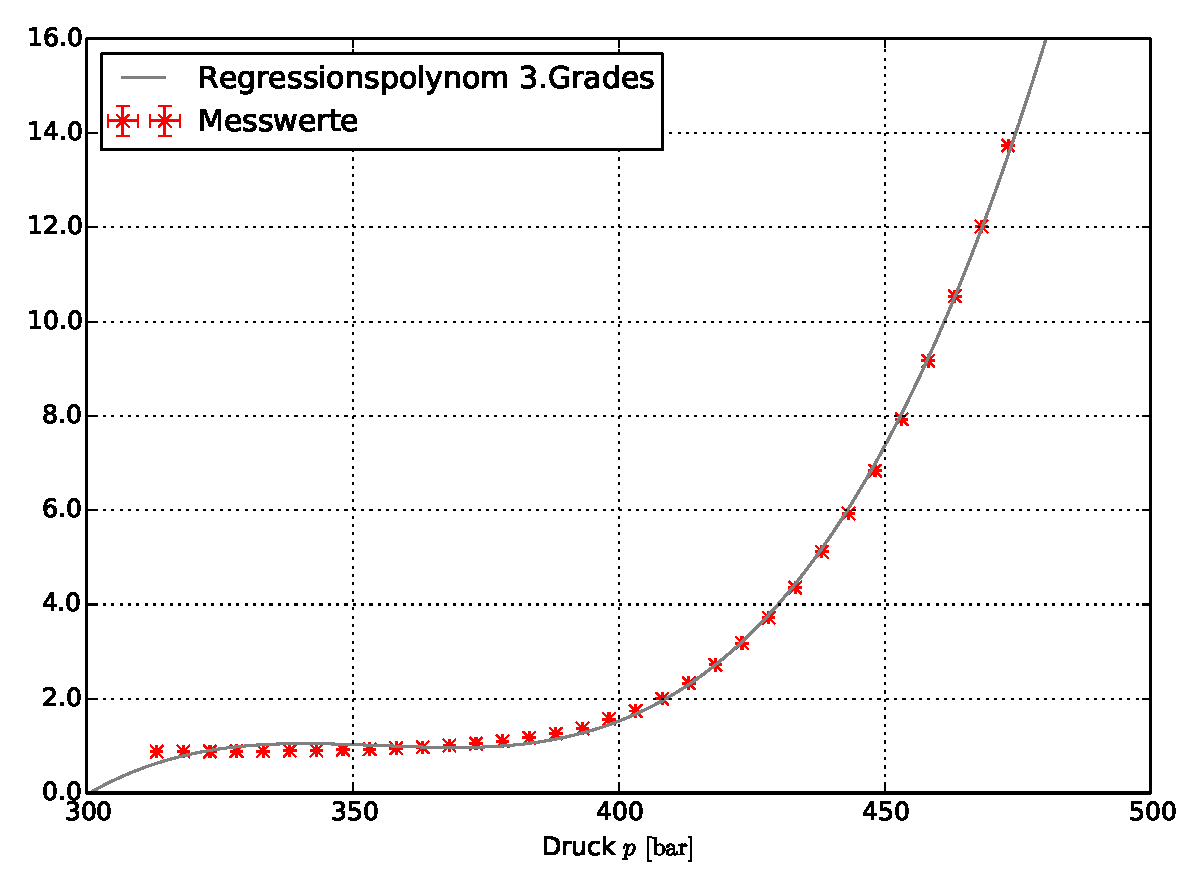
\includegraphics[scale=0.75]{Grafiken/Messreihe_2.pdf}
		\caption{Messwerte und Regressionspolynom der Form $f(x) = Ax^{3} + Bx^{2} + Cx + D$ \label{fig:pT2}}
	\end{figure}
	
	Zur Berechnung der Temperaturabhängigkeit der Verdampungswärme $L$, unter großen Drücken und Temperaturen, wird  
	zunächst \eqref{eq:Clausius} umgestellt, um die Gleichung 
	\begin{empheq}{equation}	
		L = T \cdot (V_{D} - V_{F}) \dod{p}{T}
		\label{eq:L_dpdT}
	\end{empheq}
	zu erhalten.  Der in dieser Gleichung auftretende Differentialquotient kann durch Differentiation des 
	Regressionsploynoms \eqref{eq:Reg_Pg3} mit den Parametern \crefrange{eq:Reg_Pg3a}{eq:Reg_Pg3c} 
	zu
	\begin{empheq}{equation}
		 \dod{p}{T} = 3AT^{2} + 2BT + C
		 \label{eq:dpdT}
	\end{empheq} 
	bestimmen werden.
	
	Zur Berechnung des Dampfvolumen $V_{D}$ wird mit \eqref{eq:vanderWaals} eine im Vergleich zur allgemeinen Gasgleichung
	\eqref{eq:allgGas} bessere Näherung verwendet. Durch Auflösen dieser Gleichung nach $V_{D}$ erhält man Mittels \emph{pq-Formel} 
	und mit der Konstanten 
	$ a = \SI{0.9}{\joule\cubic\meter\per\mole\squared}$ \cite{V203} 
	die zwei möglichen Volumina:
	\begin{empheq}{equation}
		V_{D_{1,2}} = \dfrac{RT}{2p} \pm \sqrt{\del{\dfrac{RT}{2p}}^{2} - \dfrac{a}{p}}
		\label{eq:Vd}
	\end{empheq} 
	Die Mittels \eqref{eq:Vd} berechneten Volumina für die Temperaturen und Drücke aus \autoref{tab:DataII} sind in \autoref{tab:Vd}
	aufgelistet. Dabei sind für die Volumina keine Fehler angegeben, da diese für das relevante Volumen $V_{D_{2}}$ von der Größenordnung
	\num{e-08} sind.
	
	\begin{table}[!h]
		\centering
		\begin{tabular}{|c|c||c|c|}
			\hline
			Volumen \enquote{+} & Volumen \enquote{-} & Volumen \enquote{+} & Volumen \enquote{-}\\
			$V_{D_{1}}\,[\si{d\meter\cubed}]$  & $V_{D_{2}}\,[\si{d\meter\cubed}]$ & $V_{D_{1}}\,[\si{d\meter\cubed}]$  & $V_{D_{2}}\,[\si{d\meter\cubed}]$ \\ \hline\hline
			\num{31.383}  & \num{0.319} & \num{14.476}  & \num{0.267} \\
			\num{31.150}  & \num{0.314} &\num{12.518}  & \num{0.264} \\
			\num{31.263}  & \num{0.310} &\num{10.802}  & \num{0.262} \\
			\num{31.040}  & \num{0.305} &\num{9.310}  & \num{0.260} \\
			\num{30.827}  & \num{0.301} &\num{8.002}  & \num{0.258} \\
			\num{30.010}  & \num{0.297} &\num{6.859}  & \num{0.256} \\
			\num{29.255}  & \num{0.293} &\num{5.959}  & \num{0.255} \\
			\num{28.294}  & \num{0.289} &\num{5.194}  & \num{0.253} \\
			\num{26.943}  & \num{0.286} &\num{4.499}  & \num{0.252} \\
			\num{25.331}  & \num{0.282} &\num{3.903}  & \num{0.252} \\
			\num{23.582}  & \num{0.279} &\num{3.403}  & \num{0.251} \\
			\num{20.810}  & \num{0.276} &\num{2.988}  & \num{0.251} \\
			\num{18.992}  & \num{0.272} &\num{2.612}  & \num{0.251} \\
			\num{16.698}  & \num{0.270} & & \\
			\hline
		\end{tabular}
		\caption{Mögliche Dampfvolumina nach \eqref{eq:Vd} \label{tab:Vd}}
	\end{table}
	
	Daraus ist ersichtlich, dass $V_{D_{1}}$ zwar Lösungen der Gleichung \eqref{eq:Vd} sind, jedoch nicht zu dem verwendeten Versuchsaufbau
	passen, da der genutzten Stahlbolzen nicht das nötige Volumen hatte um mehrere Liter Wasserdampf zu fassen.\\
	Mit dem Volumen $V_{D} := V_{D_{2}}$,den Temperaturen \autoref{tab:DataII}, den entsprechenden Differntialquotienten \eqref{eq:dpdT} und der Näherung $V_{F} << V_{D}$ erhält man 
	aus \eqref{eq:L_dpdT} die neben den Differntialquotienten in \autoref{tab:L_dpdT} dargestellten Werte für die Verdampfungswärme $L$.
	

	In \autoref{fig:L_T} sind die berechneten Verdampfungswärmen aus \autoref{tab:L_dpdT} zusammen mit 
	einem Regressionspolynom 2. Grades der Form 
	\begin{empheq}{equation}
		f(x) = Ax^{2} + Bx + C
	\end{empheq} 
	gegen die Temperaturen aus \autoref{tab:DataII} aufgetragen.
	Die mit SciPy bestimmten Regressionsparamter für dieses Polynom sind:
	\addtocounter{equation}{-1}
	\begin{subequations}
		\begin{empheq}{align}
				A &= \SI{0.334(2)}{\joule\per\mole\per\kelvin\squared}\\
				B &= \SI{-244(2)}{\joule\per\mole\per\kelvin}\\
				C &= \SI{4.47(4)e04}{\joule\per\mole}
		\end{empheq}
	\end{subequations} 
	
	\vspace{2cm}
	\begin{table}[!h]
		\centering
		\begin{tabular}{|c|c||c|c|}
			\hline
			Differentialquotient & Verdampfungswärme & Differentialquotient & Verdampungswärme\\
			$\od{p}{T}\,[\si[prefixes-as-symbols = true]{\milli\bar\per\kelvin}]$\eqref{eq:std_dp} & 
			$L\,[\si{\joule\per\mole}]$\eqref{eq:std_LT} & $\od{p}{T}\,[\si[prefixes-as-symbols = true]{\milli\bar\per\kelvin}]$ & 
			$L\,[\si{\joule\per\mole}]$\\ \hline\hline
				\num{18.8(1)}  & \num{205(1)} & \num{71.0(3)}  & \num{783(3)} \\
				\num{13.1(1)}  & \num{142(1)} & \num{85.6(3)}  & \num{946(4)} \\
				\num{8.78(7)}  & \num{96.0(8)} &\num{101.7(3)}  & \num{1128(4)} \\
				\num{5.97(4)}  & \num{65.3(4)} &\num{119.2(4)}  & \num{1327(4)} \\
				\num{4.61(1)}  & \num{50.4(1)} &\num{138.2(4)}  & \num{1545(5)} \\
				\num{4.71(2)}  & \num{51.4(2)} &\num{158.7(4)}  & \num{1782(5)} \\
				\num{6.25(5)}  & \num{68.4(5)} &\num{180.6(5)}  & \num{2038(6)} \\
				\num{9.26(8)}  & \num{101.2(8)} &\num{203.9(5)}  & \num{2315(6)} \\
				\num{13.7(1)}  & \num{150(1)} &\num{228.8(5)}  & \num{2615(6)} \\
				\num{19.6(1)}  & \num{215(2)} &\num{255.0(5)}  & \num{2938(7)} \\
				\num{27.0(2)}  & \num{296(2)} &\num{282.7(6)}  & \num{3286(7)} \\
				\num{35.8(2)}  & \num{393(2)} &\num{311.9(6)}  & \num{3660(8)} \\
				\num{46.1(2)}  & \num{506(3)} &\num{342.5(6)}  & \num{4064(8)} \\
				\num{57.8(3)}  & \num{636(3)} & & \\
			\hline
		\end{tabular}
		\caption{Differntialquotient und Temperaturabhängige Verdampfungswärme \label{tab:L_dpdT}}
	\end{table}

	
	\begin{figure}[!h]
		\centering
		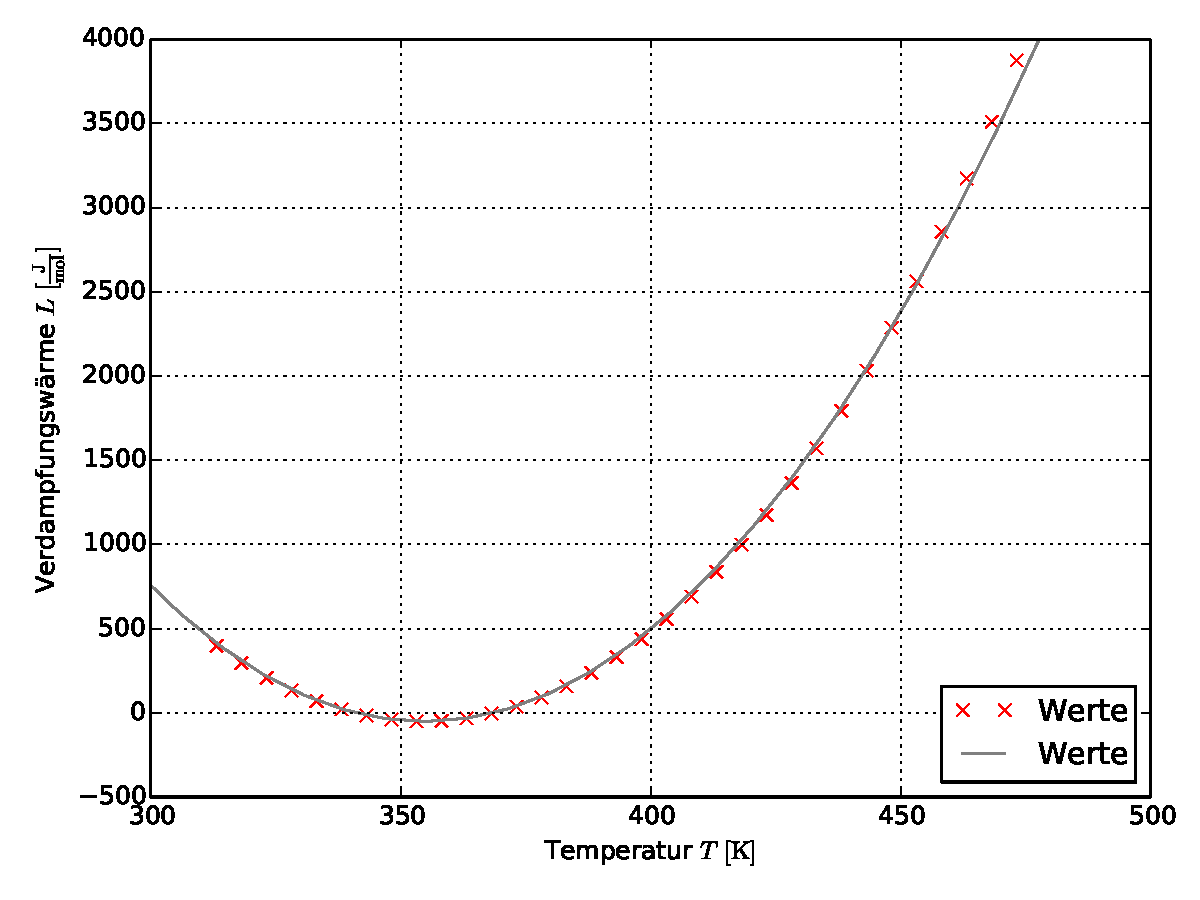
\includegraphics[scale=0.75]{Grafiken/Verlauf_LT.pdf}
		\caption{Verlauf der Verdampfungswärme unter hohen Temperaturen und Drücken}
		\label{fig:L_T}
	\end{figure}

		\newpage
		\subsection{Fehlerrechnung}\label{sec:Fehlerrechnung}
			\setcounter{equation}{0}
			\renewcommand\theequation{\Roman{equation}}
		 	
\renewcommand{\theequation}{\Roman{equation}}
\setcounter{equation}{0}

Nachfolgend sind die, Mittels Gaußscher Fehlerfortpflanzung bestimmten, Fehlergleichungen aufgelistet, die für die 
in \autoref{sec:Auswertung} angegebenen Fehler verwendet wurden.

Den Fehler der in \autoref{sec:gemittelteVerdampfungswärme} bestimmten mittleren Verdampfungswärme $L$, erhält man vereinfacht durch:
\begin{empheq}{equation}
	\sigma_{L} = R\cdot\sigma_{A}
	\label{eq:std_L}
\end{empheq}

Der Fehler der inneren Verdampfungswärme pro Molekül $L_{i}$ aus \autoref{sec:innereVerdampfungswärme} berechnet sich durch:
\begin{empheq}{equation}
	\sigma_{L_{i}} = \dfrac{L_{a} \cdot \sigma_{L}}{N_{A} \cdot \SI{1.602e-19}{\joule\per\eV}}
	\label{eq:std_Li}
\end{empheq}

Für die in \autoref{tab:L_dpdT} angegebenen Differentialquotienten $\od{p}{T} =: \dif{p}$ berechnet sich der Fehler aus:
\begin{empheq}{equation}
	\sigma_{\dif{p}}= \sqrt{9 T^{4} \sigma_{A}^{2} + 4 T^{2} \sigma_{B}^{2} + \sigma_{C}^{2} + \sigma_{T}^{2} \left(6 A T + 2 B\right)^{2}}
	\label{eq:std_dp}
\end{empheq}  

Die temperaturabhängige Verdampfungswärme aus \eqref{tab:L_dpdT} hat den Fehler:
\begin{empheq}{equation}
	\sigma_{L(T)}= \sqrt{T^{2} V_{D}^{2} \sigma_{\dif{p}}^{2} + V_{D}^{2} \dif{p}^{2} \sigma_{T}^{2}}
	\label{eq:std_LT}
\end{empheq}

	
	\newpage
	\section{Diskussion}\label{sec:Diskussion}
		In diesem Unterabschnitt werden, die durch die Auswertung erhaltenen
Größen mit Literaturwerten verglichen, um eine Aussage über deren 
Richtigkeit machen zu können. Außerdem werden diese Vergleiche noch
einmal mit dem Versuchsaufbau und der Versuchsdurchführung in Bezug
gesetzt um eventuelle Fehler aufzuzeigen, die etwaig Abweichung der 
errechneten Größen von der Realität erklären können.\\

Um die in \autoref{sec:gemittelteVerdampfungswärme} 
bestimmte, gemittelte Verdampfungswärme $L$ für Drücke 
$p < \SI{1}{\bar}$ mit dem Literaturwert $L_{lit} = 
\SI{2256}{\joule\per\g}$ \cite{Mende09}
vergleichen zu können, muss diese mit der 
Molaren Masse eines Wassermoleküls 
$M(\ce{H2O}) = \SI{18}{\g\per\mole}$\footnote{Berechnet aus den molaren Massen der Komponenten \cite{Kuchling07}} multipliziert werden, um die Verdampfungswärme pro Gramm mit 
$L =\SI{2272(22)}{\joule\per\g} $ zu erhalten.
Offensichtlich weicht die aus den Messwerten bestimmte Verdampfungswärme nur wenig vom angegebenen Literaturwert ab, diese qualitative Beobachtung lässt sich durch bilden der 
relativen Abweichung 
$ \Delta_{r} L = \tfrac{\envert{L - L_{lit}}}{L_{lit}} \approx 
\num{0.007} = \SI{0.7}{\percent}$ quantifizieren.
Dies hohe Genauigkeit zeigt, dass die Messung in diesem Teilversuch quasi
ohne systematische oder grobe Fehler erfolgte. Es sei jedoch darauf hingewiesen, dass
diese hohe Maß an Übereinstimmung nur für die zwölf verwendeten und nicht für alle 32 
aufgenommen Messwertpaare gilt, da gerade die Messwerte mit den geringsten Abweichungen 
zur Regressionsgerade für die Auswertung verwendet wurden.\\
Aus der hohen Genauigkeit der gemittelten Verdampfungswärme lässt sich darauf schließen,
dass auch die in \autoref{sec:innereVerdampfungswärme} besitmmte innere Verdampfungswärme
$L_{i}$ eine entsprechend oder zumindest vergleichbar hohe Übereinstimmung mit der Realität zeigt.\\

Die in \autoref{sec:TAbhängig} bestimmte Temperaturabhängigkeit der Verdampfungswärme
stellt ein Polynom zweiten Grades, eine nach oben geöffnete Parabel dar. 
	Diese stellt für hohe Temperaturen $ T > \SI{375}{K} $ einen plausiblen Verlauf dar,
verliert jedoch an Plausibilität für geringere Temperaturen, da ein Ansteigen der
Verdampfungswärme sowohl für größere als auch für geringere Temperaturen nicht
realistisch ist.
Der Verlauf in Form eines Polynoms zweiten Grades lässt sich durch die Bestimmung
des Differentialquotienten $\tod{p}{T}$ durch Differentiation des Regressionsploynoms 
dritten Grades aus \autoref{fig:pT2} erklären.\\


Zusammenfassend lässt sich sagen, dass die in diesem Versuch vorgenommenen Messungen 
eine, im Vergleich zur Literatur, geringe Abweichung aufwiesen, wodurch auf eine allgemein niedrige Fehleranfälligkeit des Versuchs zuschließen ist. 
\newpage
\printbibliography

\end{document}